\documentclass[12pt,letterpaper]{article}
\usepackage{graphicx,textcomp}
\usepackage{natbib}
\usepackage{setspace}
\usepackage{fullpage}
\usepackage{color}
\usepackage[reqno]{amsmath}
\usepackage{amsthm}
\usepackage{fancyvrb}
\usepackage{amssymb,enumerate}
\usepackage[all]{xy}
\usepackage{endnotes}
\usepackage{adjustbox}
\usepackage{lscape}
\newtheorem{com}{Comment}
\usepackage{float}
\usepackage{hyperref}
\newtheorem{lem} {Lemma}
\newtheorem{prop}{Proposition}
\newtheorem{thm}{Theorem}
\newtheorem{defn}{Definition}
\newtheorem{cor}{Corollary}
\usepackage{enumitem}

\newtheorem{obs}{Observation}
\usepackage[compact]{titlesec}
\usepackage{dcolumn}
\usepackage{tikz}
\usetikzlibrary{arrows}
\usepackage{multirow}
\usepackage{xcolor}
\newcolumntype{.}{D{.}{.}{-1}}
\newcolumntype{d}[1]{D{.}{.}{#1}}
\definecolor{light-gray}{gray}{0.65}
\usepackage{url}
\usepackage{listings}
\usepackage{color}

\definecolor{codegreen}{rgb}{0,0.6,0}
\definecolor{codegray}{rgb}{0.5,0.5,0.5}
\definecolor{codepurple}{rgb}{0.58,0,0.82}
\definecolor{backcolour}{rgb}{0.95,0.95,0.92}

\lstdefinestyle{mystyle}{
	backgroundcolor=\color{backcolour},   
	commentstyle=\color{codegreen},
	keywordstyle=\color{magenta},
	numberstyle=\tiny\color{codegray},
	stringstyle=\color{codepurple},
	basicstyle=\footnotesize,
	breakatwhitespace=false,         
	breaklines=true,                 
	captionpos=b,                    
	keepspaces=true,                 
	numbers=left,                    
	numbersep=5pt,                  
	showspaces=false,                
	showstringspaces=false,
	showtabs=false,                  
	tabsize=2
}
\lstset{style=mystyle}
\newcommand{\Sref}[1]{Section~\ref{#1}}
\newtheorem{hyp}{Hypothesis}

\title{Answer Key: Problem Set 4}
\date{Jeffrey Ziegler}
\author{Applied Stats II}

\begin{document}
	\maketitle
	
	\section*{Instructions}
	\begin{itemize}
		\item \textit{Please show your work! You may lose points by simply writing in the answer. If the problem requires you to execute commands in \texttt{R}, please include the code you used to get your answers. Please also include the \texttt{.R} file that contains your code. If you are not sure if work needs to be shown for a particular problem, please ask.}
			\item \textit{Your homework should be submitted electronically on GitHub in \texttt{.pdf} form.}
			\item \textit{This problem set is due before 23:59 on Friday April 10, 2026. No late assignments will be accepted.}
	\end{itemize}
	\vspace{.25cm}
	
	\section*{Question 1}
	\vspace{.25cm}
	\noindent \emph{We're interested in modeling the historical causes of child mortality. We have data from 26855 children born in Skellefteå, Sweden from 1850 to 1884. Using the "child" dataset in the \texttt{eha} library, fit a Cox Proportional Hazard model using mother's age and infant's gender as covariates. Present and interpret the output.}\\
	
	First, let's estimate our Cox proportional hazard model:
	\vspace{.25cm}
	\lstinputlisting[language=R, firstline=39,lastline=43]{../answer_key/PS4_answerKey.R} 
	\vspace{.25cm}
	\noindent Looking at Table~\ref{table:coefficients}, we can interpret the estimated coefficient for gender as the logged hazard ratio of boys with respect to girls for infants with mothers of the same age. If we exponentiate the estimated coefficient of gender (exp(coef)= 0.923), we see that boys are, on average, about 8\% less likely to survive than girls with mothers of the same age (HR $< 1$ = reduction in the hazard). Looking at the age coefficient, we can see that having an older mother (holding infant gender constant) is also a “poor prognostic factor” that increases the risk of death. More specifically, a one unit increase in mother's age is associated with an increase in the logged hazard ratio for infants of the same gender.
	
		\begin{table}[h!]
		\caption{\footnotesize Cox Proportional Hazard model results}
		\vspace{.25cm}
		\label{table:coefficients}
		\centering
		\begin{adjustbox}{width=.3\textwidth}
			\begin{tabular}{l c}
				\hline
			m.age       & $0.01^{***}$ \\
            & $(0.00)$     \\
sex\_female   & $-0.08^{**}$ \\
            & $(0.03)$     \\
\hline
AIC         & $113010.97$ \\
\# events & $5616$     \\
N   & $26574$    \\

				\hline
				\multicolumn{2}{l}{\footnotesize{$^{***}p<0.001$; $^{**}p<0.01$; $^{*}p<0.05$}}
			\end{tabular}
		\end{adjustbox}
	\end{table}
	
	\noindent To visually investigate the relationship between gender and mothers’ age further, we can see that in Figure 1, children generally survive longer when they have younger mothers (which may be symptomatic of access to healthcare and economic class). Moreover, we can see that girls generally survive longer than boys.
	
		
	\begin{figure}[h!]\centering
		\caption{\footnotesize Predicted survival probability by gender and mother age.}
		\label{fig:coxph}
				\vspace{.25cm}
		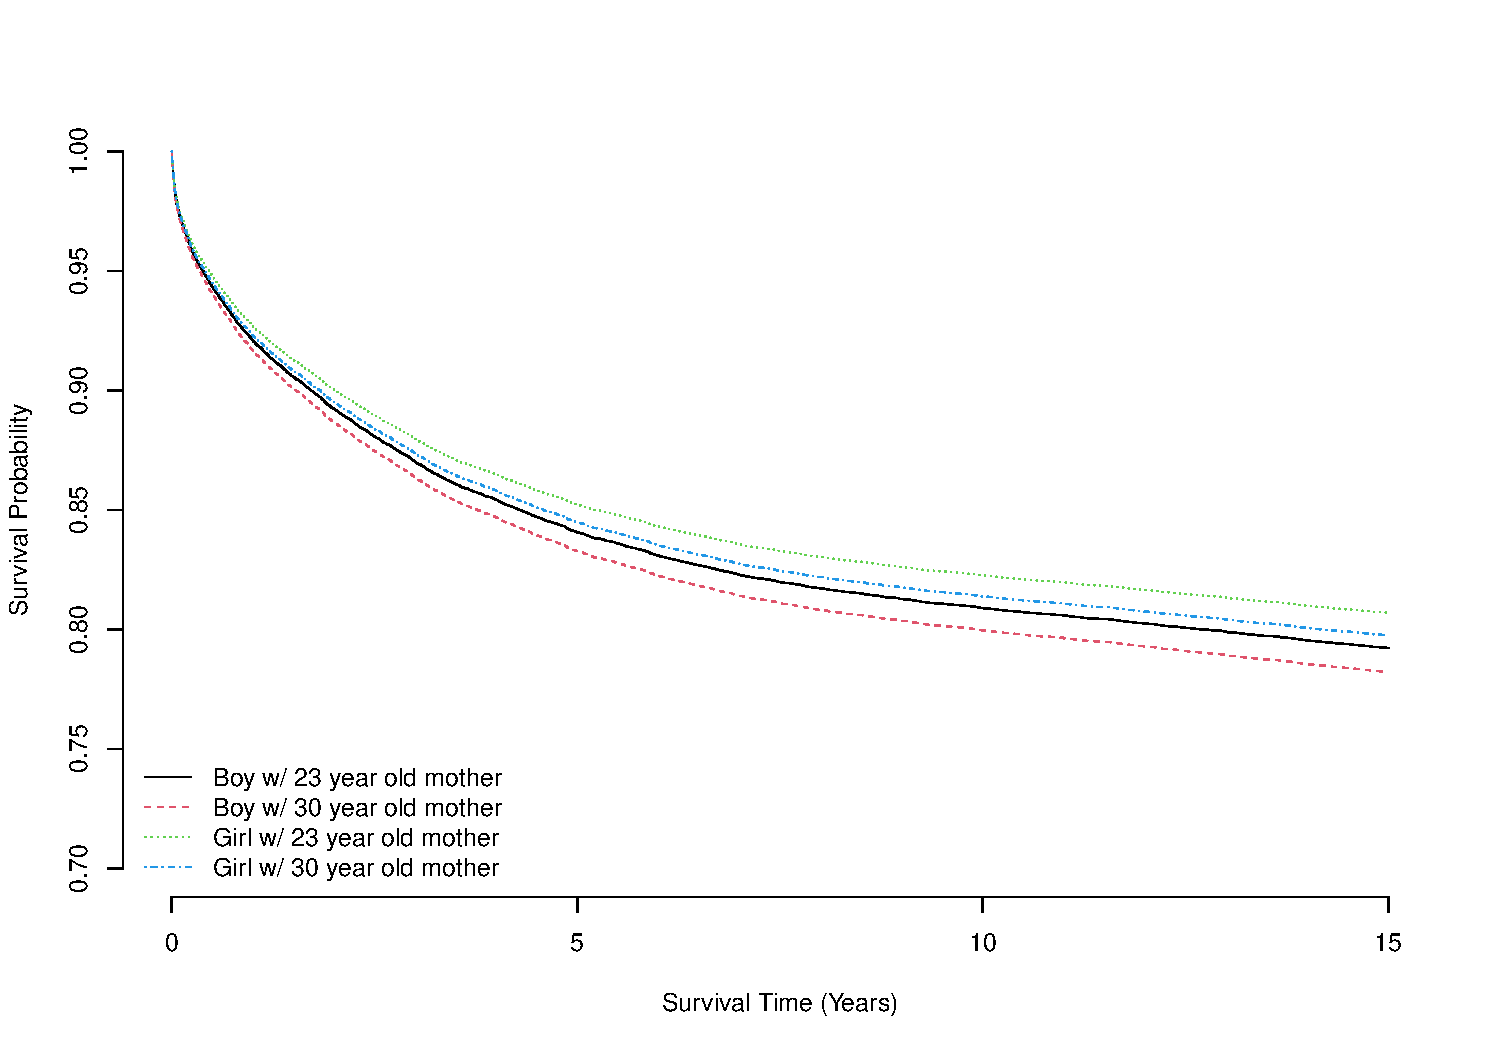
\includegraphics[width=.95\textwidth]{figure1.pdf}\\
	\end{figure}

	\section*{Question 2}
	\vspace{.25cm}
	\noindent \emph{We want to estimate how the amount of damage caused by a disaster relates to (1) whether disaster relief is provided and (2) the amount of relief that is provided  conditional on a donation occurring when a disaster hits a given country. Estimate a Heckman selection model using the \texttt{disasters\_response} data on \href{https://raw.githubusercontent.com/ASDS-TCD/StatsII_2026/refs/heads/main/datasets/disaster_response.csv}{GitHub} in which \texttt{binContribution} is the outcome for the selection equation, and \texttt{originalContributionMillionUSDLogged} is the outcome for the second equation. Use \texttt{occurrences  + deathsEM + normalizedDamageEMLogged} as your input variables for both equations. Present and interpret the output.}\\
	
	\noindent Taken together, the results in Table~\ref{table:heckman} indicate that disasters with more severe observable characteristics (such as an greater number of occurrences, resulting deaths, and greater damage) are more likely to trigger any relief, but among disasters that do receive aid, those same observed characteristics do not clearly predict the size of the aid package. The  inverse Mills ratio is negative and statistically significant, which shows that a simple regression on only the funded cases would likely be biased, so the Heckman correction is useful in this context.\\
		
	\noindent Specifically, regarding the selection equation (remember, "holding all covariates constant" and these are "average effects"):
	\begin{itemize}
		\item A one-unit increase in \textit{occurrences} is associated with a 0.0192 increase in the latent index for receiving any contribution.
		\item A one-unit increase in \textit{deathsEM} is associated with a 0.0115 increase in the latent index for receiving any contribution.
		\item A one-unit increase in \textit{logged normalized damage} is associated with a 0.0211 increase in the latent index for receiving any contribution.
	\end{itemize}

	\noindent Interestingly, all of these coefficients are estimated to have statistically non-zero relationships with the likelihood of selection. Note, since this first stage selection is a probit model, I mean this in the qualitative sense (literally the z-score of the normal cumulative distribution function), rather than a direct change in probability or log-odds of receiving a donation.\\
	
	\noindent Regarding the outcome equation, a one-unit increase in one of our predictors is associated with a $\hat{\beta}$ change in logged contribution amount, conditional on receiving aid (again, "holding all covariates constant" and these are "average effects"). In none of these instances is the estimated relationship statistically non-zero.
	
	\begin{table}
		\begin{center}
			\caption{\footnotesize Estimated coefficients from selection and outcome equation.}
			\begin{tabular}{l c}
				\hline
				& Model 1 \\
				\hline
				S: (Intercept)              & $-1.3020^{***}$ \\
				& $(0.0180)$      \\
				S: occurrences              & $0.0192^{***}$  \\
				& $(0.0017)$      \\
				S: deathsEM                 & $0.0115^{***}$  \\
				& $(0.0007)$      \\
				S: normalizedDamageEMLogged & $0.0211^{***}$  \\
				& $(0.0009)$      \\
				O: (Intercept)              & $9.7663$        \\
				& $(6.0440)$      \\
				O: occurrences              & $-0.0863$       \\
				& $(0.0549)$      \\
				O: deathsEM                 & $-0.0330$       \\
				& $(0.0257)$      \\
				O: normalizedDamageEMLogged & $-0.1142$       \\
				& $(0.0623)$      \\
				invMillsRatio               & $-6.3129$       \\
				& $(3.4204)$      \\
				sigma                       & $5.9924$        \\
				& $$              \\
				rho                         & $-1.0535$       \\
				& $$              \\
				\hline
				R$^2$                       & $0.0546$        \\
				Adj. R$^2$                  & $0.0534$        \\
				Num. obs.                   & $49096$         \\
				Censored                    & $45848$         \\
				Observed                    & $3248$          \\
				\hline
				\multicolumn{2}{l}{\scriptsize{$^{***}p<0.001$; $^{**}p<0.01$; $^{*}p<0.05$}}
			\end{tabular}

			\label{table:heckman}
		\end{center}
	\end{table}

\end{document}
